In this section, we learn about matrices.  We discuss how to input matrices, alter existing matrices, and use them in computations.  We use such functions as inverse, determinant, and transpose.  We show how to select specific rows, columns or entries in a matrix and how to use matrices in solving systems of equations.  

\section{Mathcad: Matrix Definition}\label{sec:Mathcad_matrices}

\index{Mathcad!Matrices}
\index{Mathcad!Toolbars!Matrix}
We begin with showing how to input a matrix into a Mathcad worksheet.\\

\noindent \large \textsf{\textbf{Entering matrices and basic operations}} \normalsize\\

First, open the matrix toolbar with File $>$ Toolbars $>$ Matrix:

\begin{center}
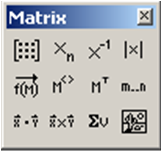
\includegraphics{figures/mathcad_matrix_toolbar.png}
\end{center}

and select the  
\includegraphics{figures/mathcad_insert_matrix_dialog_box_button1.png} button in the upper left corner to launch the ``Insert Matrix'' dialog box:

\begin{center}
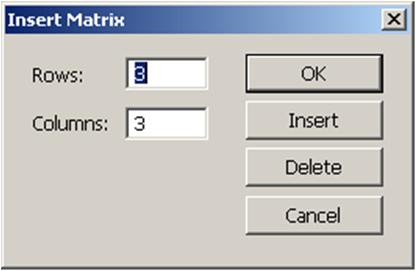
\includegraphics{figures/mathcad_insert_matrix_dialog_box.png}
\end{center}

Input the desired number of rows and columns and click on ``Insert''. This creates a template of the correct size that you can use for your matrix.  Note that as you enter numbers in the black boxes, you can move to the next black box with the Tab key, or between the entries with the arrow keys.

Let's try an example.

Find the sum and the product of the matrices 
\[
\left[
\begin{array}{lll}
1 & 2 & 4\\
0 & -1 & 7\\
1 & 1 & 1
\end{array}
\right]
\quad
{\rm and}
\quad
\left[
\begin{array}{lll}
2 & 0 & 0\\
3 & -3 & 1\\
7 & 8 & 9
\end{array}
\right]
\]

We input the matrices and store them as variables \textbf{a} and \textbf{b}.  Here we see them partially filled in:\\
\\
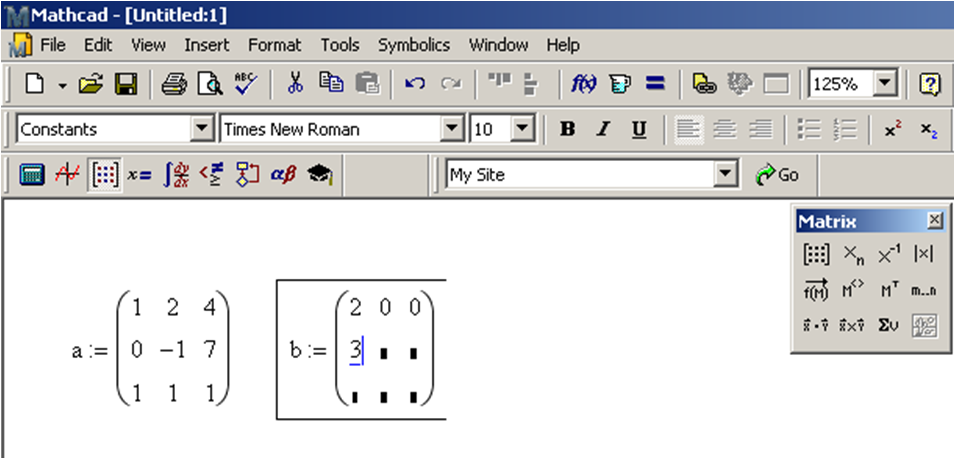
\includegraphics[scale=.75]{figures/mathcad_matrix_example1a.png}


The sum and product of the resulting matrices are done using the standard plus $+$ and times $\ast$ (which appears as a dot): \\
\\
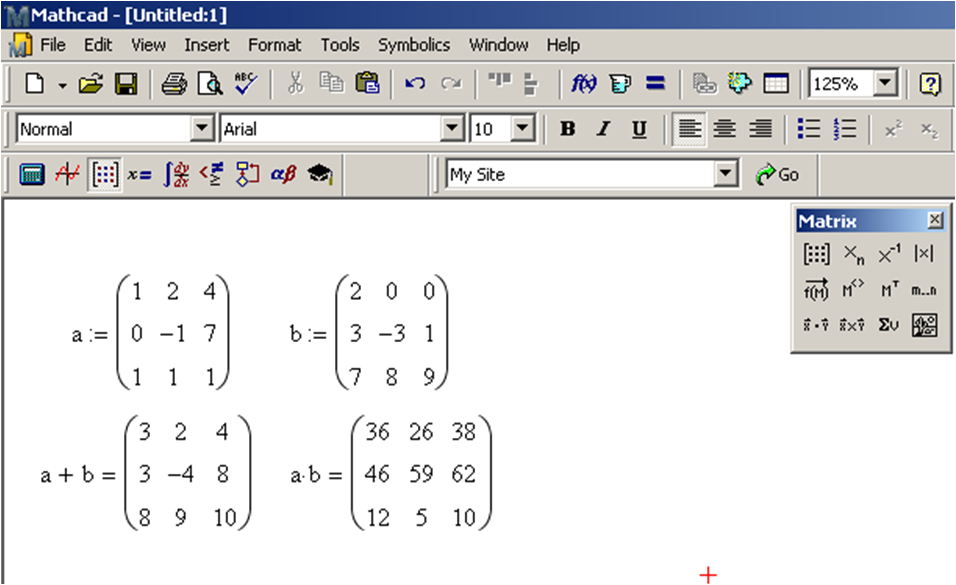
\includegraphics[scale=.75]{figures/mathcad_matrix_example1b.png}

\section{Mathcad: Editing Matrices}\label{sec:Mathcad_matrices2}

There are many different ways to alter an existing matrix.  In these examples, note that we don't use the variable \textbf{c} since that is the built-in variable for the speed of light (although we could redefine \textbf{c}, there is no need to do so and it is generally a good idea not to overwrite the built-in variables).\\

\index{Mathcad Functions!\tnr{augment}}
$\bullet$ \textbf{Augmenting a matrix by another matrix}  (side-by-side)\\

If two matrices have the same number of rows, we can create a new matrix with the command \textbf{augment}:\\
\\
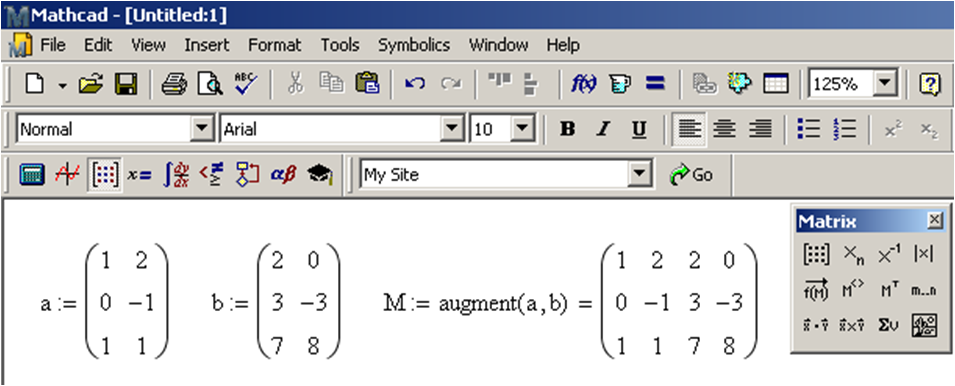
\includegraphics[scale=.80]{figures/mathcad_matrix_augment.png}

\newpage
$\bullet$ \textbf{Stacking two matrices}\\

\index{Mathcad Functions!\tnr{stack}}
If two matrices have the same number of columns, we can create a new matrix with the command \textbf{stack}:\\
\\
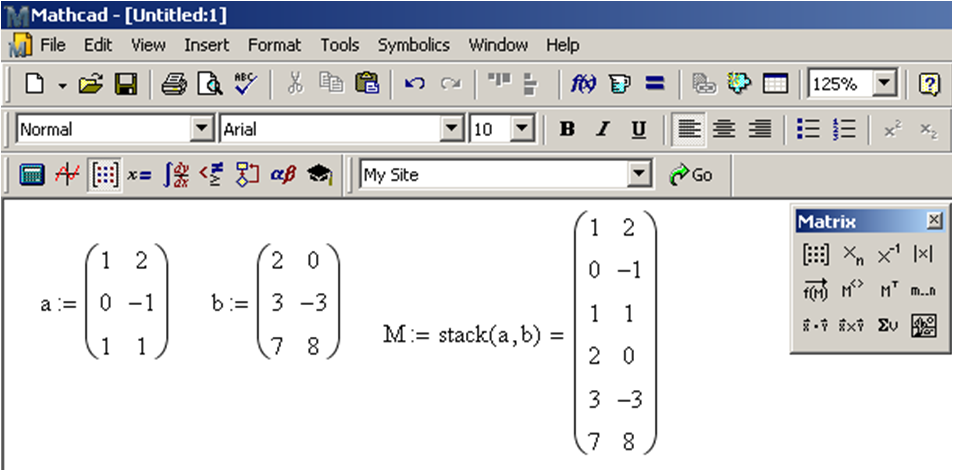
\includegraphics[scale=.7]{figures/mathcad_matrix_stack.png}

\index{Mathcad!Insert$\backslash$Delete Matrix Row or Column}
$\bullet$ \textbf{Inserting a row or column}\\

To insert new row(s) or column(s) to an existing matrix, select an entry of the matrix.  The inserted row(s) or column(s) will appear below or to the right of the selected entry.  Then click the 
\includegraphics{figures/mathcad_insert_matrix_dialog_box_button1.png} button.  Change the entries for the desired number of rows and columns and click ``Insert''.  If you only want to insert a single row, set the number of columns to zero.  If you only want to insert a single column, set the number of rows to zero.

\begin{center}
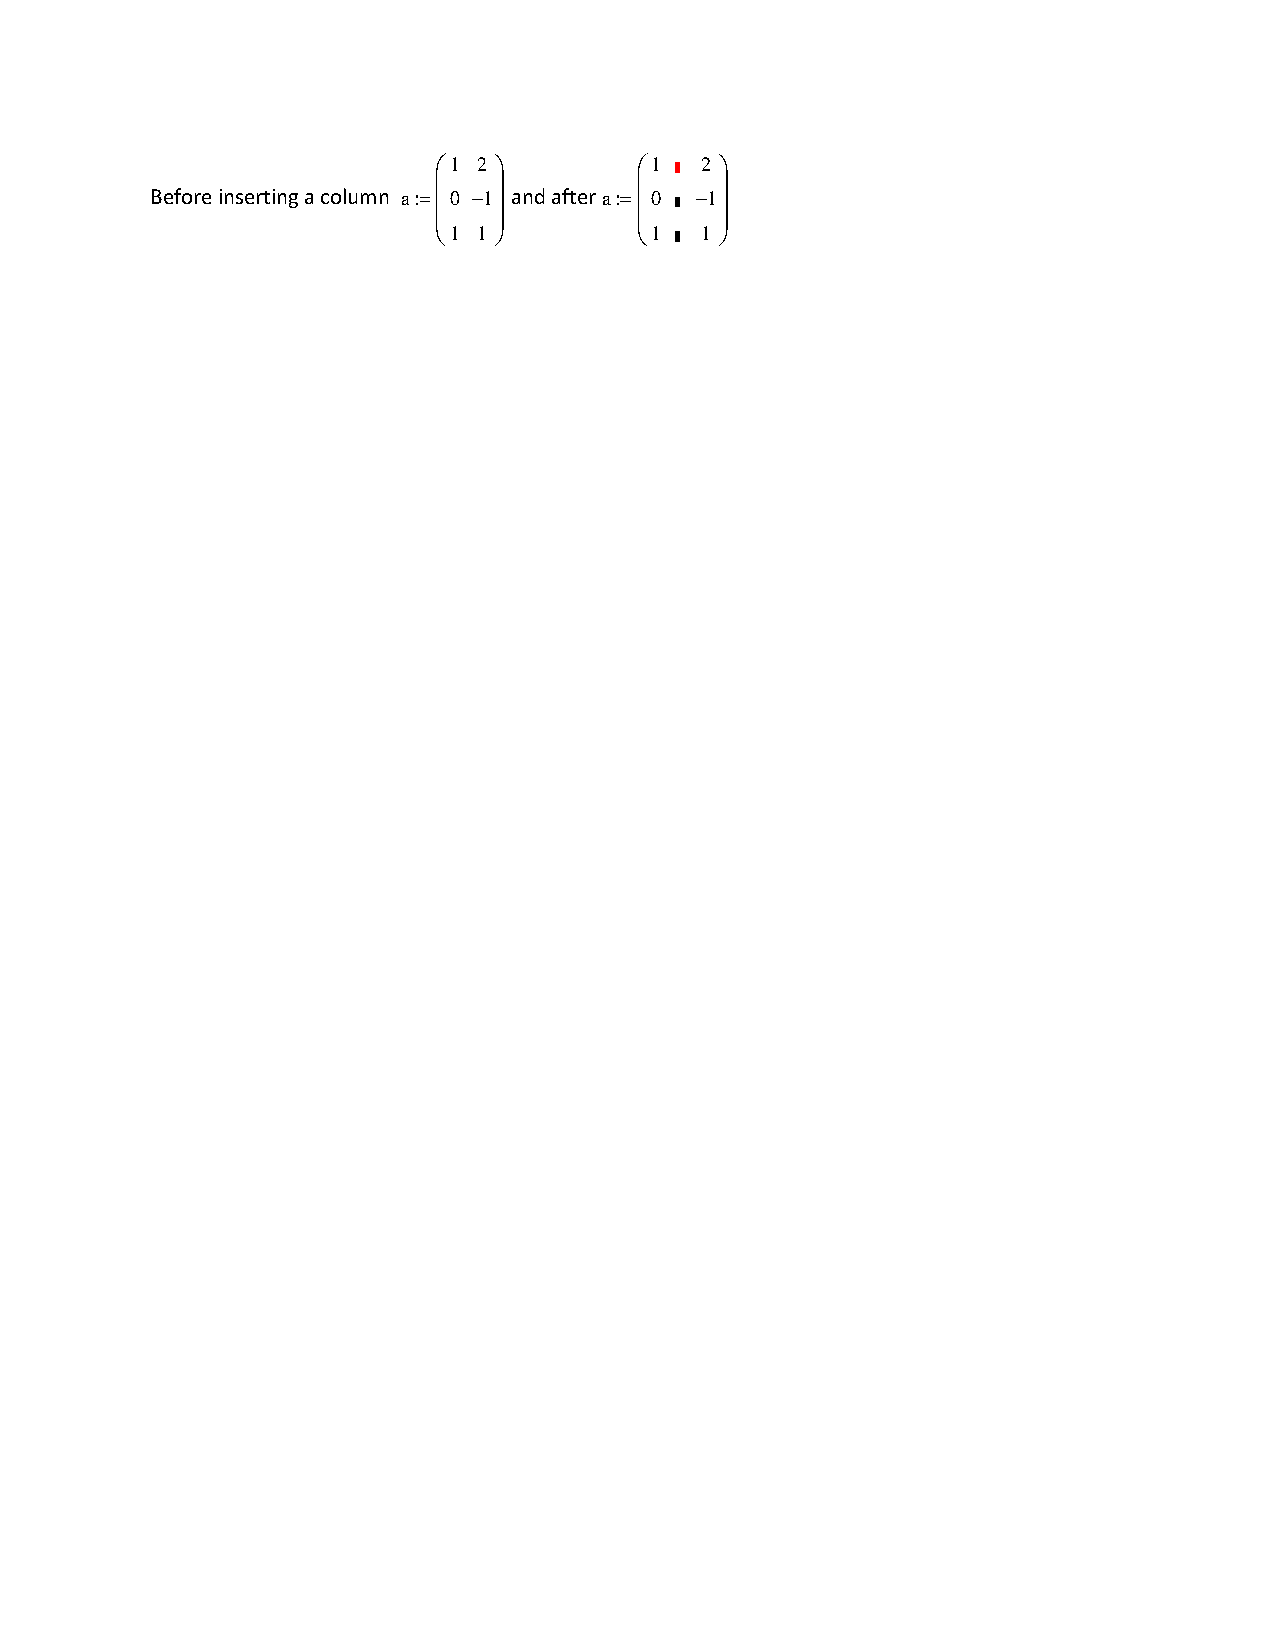
\includegraphics[bb=3in 9in 3in 10.2in]{figures/mathcad_matrix_new_column.pdf} %Mathcad copied to Word, saved as pdf, guess bounding box size
\end{center}

New rows are inserted below a highlighted row and columns are inserted to the right of a highlighted row. If you want to insert a new first row or column, you need to select the \underline{whole} matrix before using the 
\includegraphics{figures/mathcad_insert_matrix_dialog_box_button1.png} button and making the insertion.\\


$\bullet$ \textbf{Deleting a row or column}\\

The process of deleting rows or columns is similar to making insertions. To delete rows or columns from an existing matrix, select an entry of the matrix.  The deleted rows) or columns will contain that entry and delete rows below and columns to the right.  Then click the 
\includegraphics{figures/mathcad_insert_matrix_dialog_box_button1.png} button.  Change the entries for the desired number of rows and columns and click ``Delete''.  \\

\section{Mathcad: Referencing Parts of Matrices}\label{sec:Mathcad_matrices3}

%\index{Mathcad Functions!\tnr{ORIGIN}}
%\noindent \large \textsf{\textbf{Finding submatrices}} \normalsize\\

Sometimes you may need to use part of a matrix: an entry, a row, a column, or a submatrix inside another matrix.  You must be very careful in referencing parts of a matrix, since the default for the starting index is zero!!  This means that the ``first'' row of a matrix is referenced as if it was ``row zero''.  The start index is stored in a variable called \textbf{ORIGIN} and can be changed for a worksheet in two ways, either by using Tools $>$ Worksheet Options (and changing \textbf{ORIGIN}) or by typing ORIGIN:=1 at the top of the worksheet.\\
%use the command submatrix(A, startrow,endrow,startcolumn,endcolumn)

\index{Mathcad! Reference matrix entries}
$\bullet$ \textbf{Referencing one entry in a matrix}\\

To select a single number out of an existing matrix, one can use the ``subscript'' operator from the matrix toolbar (the $\textbf{x}_\textbf{n}$ button), or with the $[$ key.  Here we select the entry in the 2nd row and 2nd column by resetting the \textbf{ORIGIN} to 1 and defining \textbf{b} from the matrix \textbf{a}.\\
\\
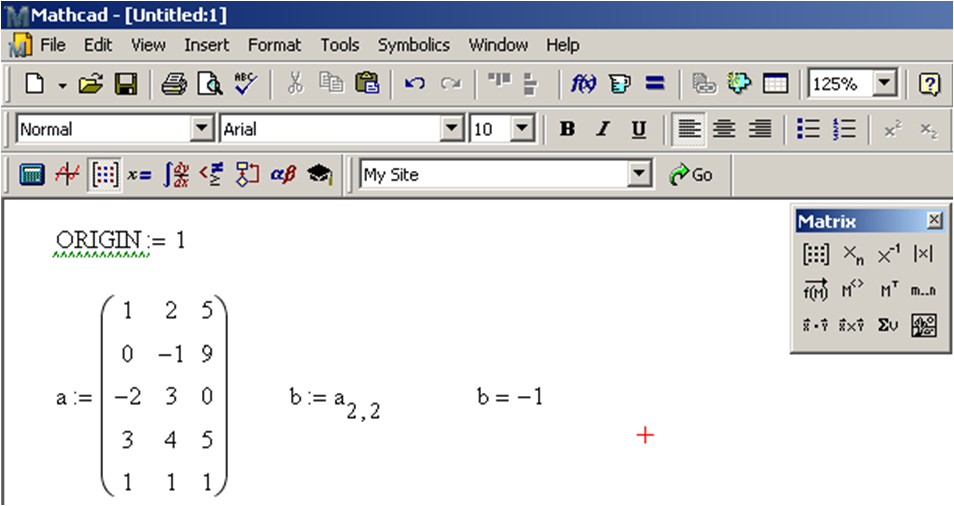
\includegraphics[scale=.7]{figures/mathcad_matrix_subscript.png}

Note that if a matrix has only one column (a ``column vector'') or a single row (a ``row vector'') then only one subscript is necessary.\\
\\
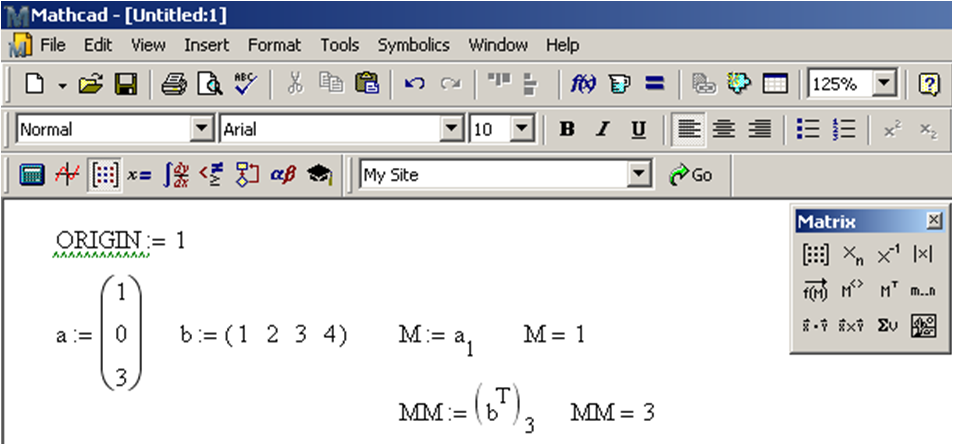
\includegraphics[scale=.7]{figures/mathcad_matrix_column_vector.png}\\

\index{Mathcad!Reference matrix column}
$\bullet$ \textbf{To reference one column in a matrix}\\

To select a single column out of an existing matrix, one can use the ``Column'' operator from the matrix toolbar (the $\textbf{M}^{<>}$ button), or with the keyboard shortcut Ctrl $+ 6$.  Here we select the 2nd column by resetting the \textbf{ORIGIN} to 1 and defining \textbf{b} from the matrix \textbf{a}.\\
\\
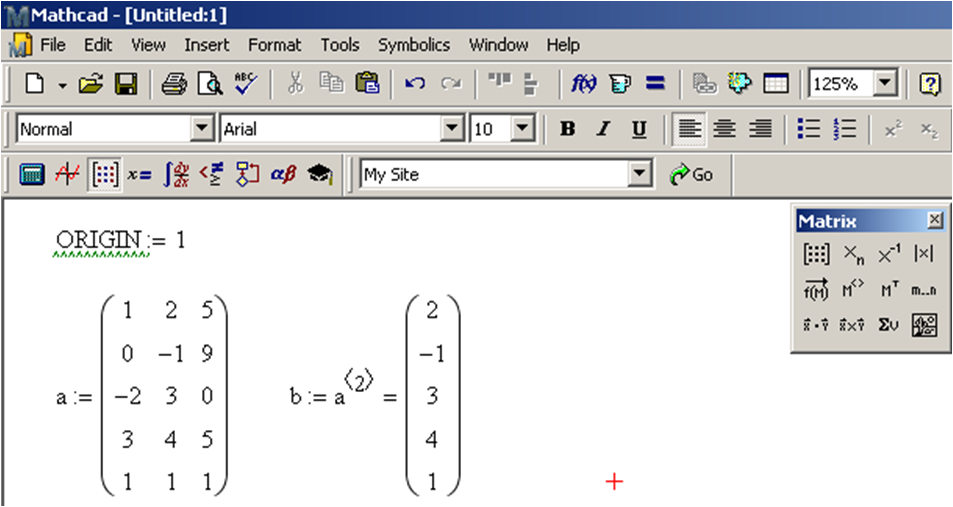
\includegraphics[scale=.7]{figures/mathcad_matrix_column.png}

\index{Mathcad!Reference matrix row}
$\bullet$ \textbf{To reference one row in a matrix}\\

It is trickier to select a single row out of an existing matrix.  One must use a combination of the ``Transpose'' operator (that switches rows and columns) together with the ``Column'' operator.  The transpose operation on the matrix toolbar is the $\textbf{M}^{\textbf{T}}$ button and can also be created with the keyboard shortcut Ctrl $+ 1$.  Here we select the 2nd row by resetting the \textbf{ORIGIN} to 1 and defining \textbf{b} from the matrix \textbf{a}.  Typing this is a bit tricky.  The exact sequence of keys is 

\[
\textbf{b} \quad : \quad \textbf{a} \quad (\text{Ctrl} + 1) \quad (\text{Ctrl} + 6) \quad 2 \quad (\text{spacebar}) \quad (\text{Ctrl} + 1) \quad = \\
\]
\\
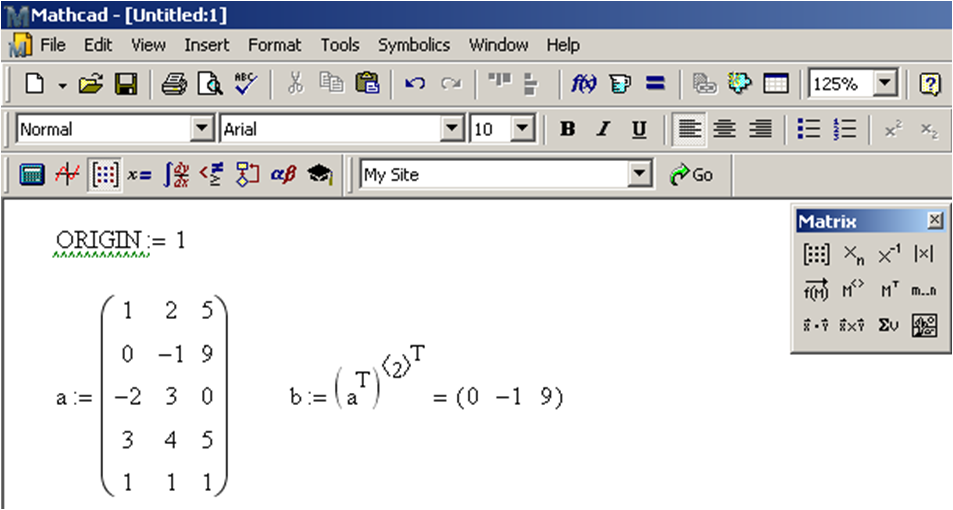
\includegraphics[scale=.75]{figures/mathcad_matrix_row.png}\\

\index{Mathcad Functions!\tnr{submatrix}}
$\bullet$ \textbf{To reference a submatrix}\\

Selecting a submatrix from an existing matrix is done only through the command \textbf{submatrix}.  Here we select the submatrix using the 2nd through 4th rows and 2nd through 3rd columns from the matrix \textbf{a}.  \\
\\
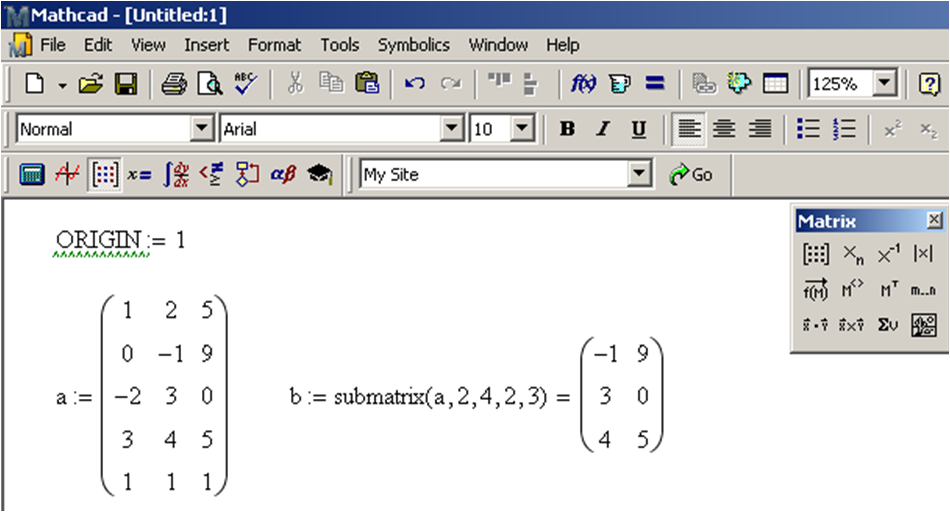
\includegraphics[scale=.75]{figures/mathcad_matrix_submatrix.png}\\

\section{Mathcad: Solving Systems of Linear Equations}\label{sec:Mathcad_matrices4}

%$\bullet$ \textbf{Solving systems of linear equations}\\

Suppose we have the following system of linear equations.

\[
\begin{array}{rl}
3w-x+y+z & = 3\\
-x-y+3z & = 1\\
5w+3x-y-z & = -1\\
2w+2x-y & = 0\\
\end{array}
\]

The goal is to solve them simultaneously for the variables $w,x,y$ and $z$.  Assuming that there is exactly one answer (i.e. one quadruple for $w,x,y,z$) then there are many ways to do this.  Here we use rref, lsolve and the matrix inverse as examples.\\

\index{Mathcad Functions!\tnr{rref}}
$\bullet$ \textbf{rref}\\

The command rref is short for ``reduced row echelon form.'' Through a process called Gaussian elimination the matrix of coefficients (on $w,x,y,z$) augmented by the matrix of constants (the numbers on the right of the equals signs) is reduced to a matrix of zeros and ones (the ``identity matrix'') together with the solution (in the last column).  In the matrix \textbf{a}, we store the cofficients for $w$ in the first column, $x$ in the second column, $y$ in the third column, $z$ in the fourth column and the constants in the fifth column.  If a variable does not occur in an equation, a zero is in the corresponding entry of the matrix \textbf{a}. \\
\\
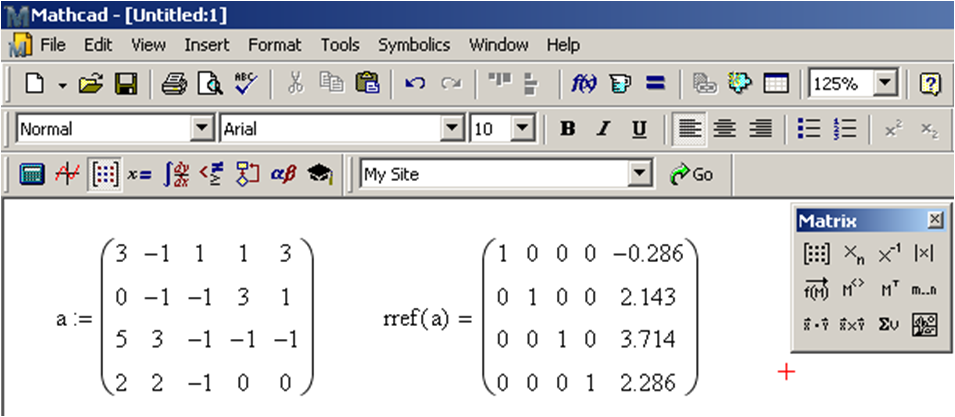
\includegraphics[scale=.75]{figures/mathcad_matrix_rref.png}\\

The last column indicates that the only solution to the system of equations is $w=-0.286, x=2.143, y=3.714 ,z=2.286$ to three place decimal accuracy. Recall, for more decimal places, select Format $>$ Result or simply double click the equation.\\

\newpage
\index{Mathcad Functions!\tnr{lsolve}}
$\bullet$ \textbf{lsolve}\\

To use the command \textbf{lsolve}, we need two separate matrices, one with the coefficients of $w,x,y,z$ and one with the constants to the right side of the equals sign. We could input this from scratch or practice referencing them from the matrix \textbf{a} above.  Here is the syntax for how to use the \textbf{lsolve} command.\\
\\
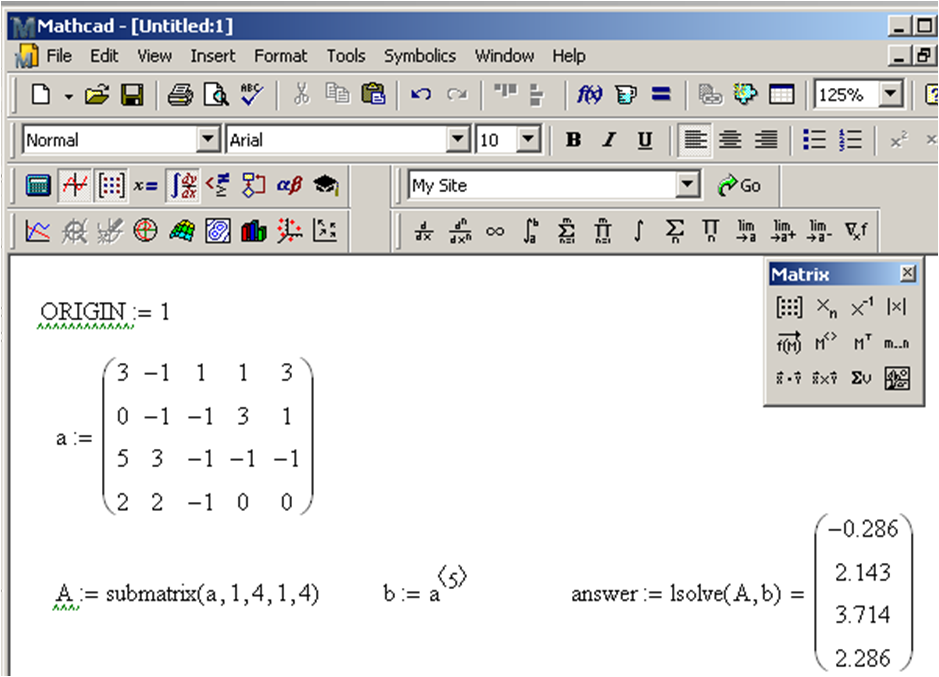
\includegraphics[scale=.75]{figures/mathcad_matrix_lsolve.png}\\

The variable \tnr{answer} contains the only solution to the system of equations as $w=-0.286, x=2.143, y=3.714 ,z=2.286$.\\
\\
$\bullet$ \textbf{Using the matrix inverse}\\

The setup for the using the inverse of a matrix is similar as for using \textbf{lsolve}.  We need the coefficient matrix of $w,x,y,z$ and the constant matrix.  The inverse of a matrix is found by typing the name of the matrix and then selecting the $\textbf{x}^{\textbf{-1}}$ button.  When entering the equation for the variable \textbf{answer}, make sure that \textbf{b} is multiplying correctly.  Here is the sequence of commands:

\[
\textbf{answer} \quad : \quad \textbf{A} \quad \text{x}^{-1} \quad (\text{spacebar}) \quad (\text{spacebar}) \quad \textbf{b} \quad = 
\]
\\
\hspace{-.2in} 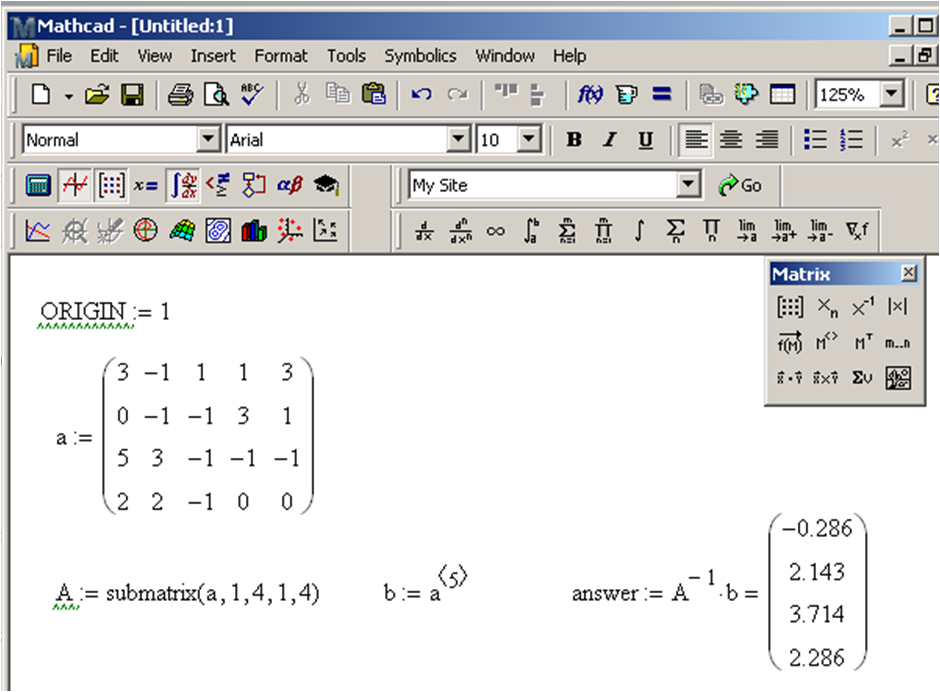
\includegraphics[scale=.75]{figures/mathcad_matrix_inverse.png}\\
\\
The variable \tnr{answer} contains the only solution to the system of equations as $w=-0.286, x=2.143, y=3.714 ,z=2.286$.\\
\\

You might be wondering ``if there are several methods to find the solution, then which technique should you use?''
The answer is (of course) more complex than we will go into here, but leave it to say that some techniques are faster or more accurate than others.  In fact if a system is either ``non-square'' (has a different number of equations and variables) or the coefficient matrix is ``singular'' (look it up) then the \textbf{lsolve} and inverse techniques don't work and in this case the system of equations either has no solution (``inconsistent'') or has infinitely many solutions (``underdetermined'').  Ok, enough theory.  

\newpage
\printexercises{exercises/14_exercises}

%\begin{adjustwidth}{-60pt}{-60pt}
\begin{adjustwidth}{-20pt}{-20pt}%
\sffamily 
\exinput{exercises/14_ex_05}
\rmfamily
\end{adjustwidth}
